\section{Proposed Method}
The model proposed in this paper consists of two modules. The first module is a feature extractor which is enabled to extract features indicating the strength of the current price trend in the near future. The second module is an actor-critic based model which selects a single coin to buy and hold until the next investment interval based on the uncertainty about the price trends of each coin extracted by the first module. 

Figure \ref{fig:arch} illustrates the architecture of the model presented in this study. The model is built based on the concept of disentangled representation learning, where a feature extractor is trained to extract features from the historical price data of each coin. These extracted features are then combined and fed into an actor-critic model to select a single coin from the available options in the market. It is important to note that the portfolio proposals in this research consist of only one coin, and no combination of coins is considered. This constraint is imposed to enhance the clarity of the model's investigation and facilitate comparisons with the existing models in the field.


%In the context of stock trading, we approach the complex task by decomposing it into two distinct components: leveraging pre-trained deep learning models for portfolio management as expert models, and introducing a novel Model Switching Agent (MS Agent) designed to dynamically select the most suitable expert model based on the current state of the environment and the performance of each expert model. This two-pronged approach aims to enhance the adaptability and effectiveness of the overall trading system by intelligently switching between expert models to optimize decision-making in response to changing market conditions. Figure \ref{fig:arch} illustrates the structure of this idea.

\begin{figure}[H]
	\centering
	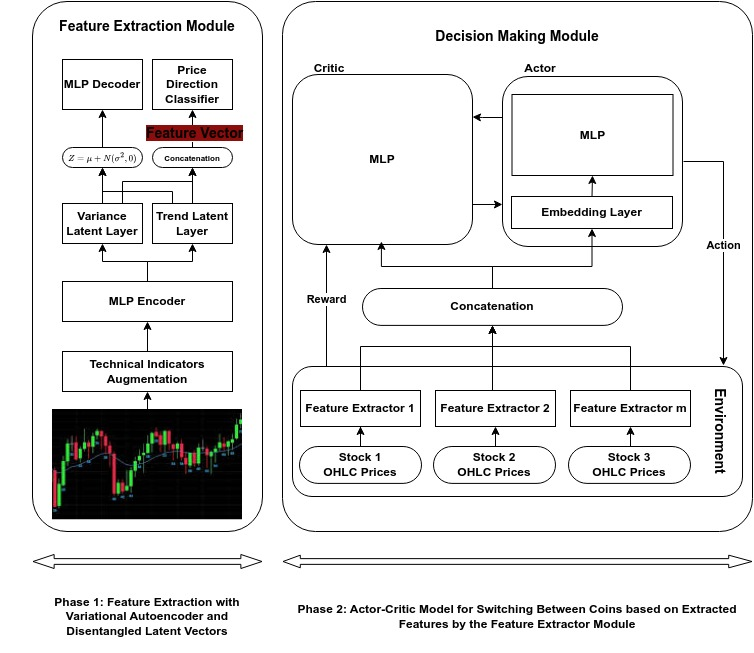
\includegraphics[scale=0.6]{./NewArch.jpg}
	\caption{Structure of the Model Switching approach for stock trading}
	\label{fig:arch}
\end{figure}


\subsection{Feature Extraction}

Disentangled representation learning is a powerful technique in machine learning that aims to learn representations of data where different factors of variation are separated into distinct and interpretable components. This can be particularly useful in time series data, where multiple underlying processes may be present and need to be disentangled for better understanding and analysis.

Let's consider a time series dataset $X = \{x^1, x^2, ..., x^t\}$, where $x^i$ represents the observation at time step $i$. The goal of disentangled representation learning on time series is to learn a set of latent variables $Z = \{z_1, z_2, ..., z_K\}$ that capture the underlying factors of variation in the data. These latent variables should be disentangled, meaning that each $z_k$ represents a different aspect of the data that is independent of the others.

Given the assumption of independence among the generating factors, the task of disentangled representation learning in a dimension-wise manner aims to encode the information pertaining to these generating factors by means of a latent vector of lower dimensionality - as a compact representation of the high-dimensional observations. The relationship between the observations and the latent vectors can be formally characterized by their joint distribution

\begin{align}
	p_\theta(x,z) &= p_\theta(x|z) p_\theta(z) \label{eq:1}\\
	p_\theta(z) &= N(z|0, \sigma^2 I) \label{eq:2}
\end{align}
where $\theta$ denotes the set of parameters of the feature extractor model and the prior distribution $p(z)$ is typically assumed to be a multidimensional Gaussian distribution with the same variance in all directions 


One common approach to achieve disentangled representation learning on time series data is through Variational Autoencoders (VAEs) (\citet{duan2019unsupervised}, \citet{li2022towards}, and \citet{li2021learning}). VAEs are generative models that learn a probabilistic mapping between the observed data and the latent variables. By introducing a prior distribution over the latent variables, VAEs can learn disentangled representations by encouraging the latent variables to capture independent factors of variation in the data.

In the first module of the proposed method, we utilize a VAE structure to capture the underlying distribution of the data and extract disentangled representations for uncertainty measurement in stock portfolio management. The VAE is designed to learn a latent space that separates different factors of variation in the data, enabling us to better understand and quantify the uncertainty associated with our model's predictions.

The VAE consists of an encoder network that maps input data (e.g., historical stock prices, market indicators) to a latent space representation, and a decoder network that reconstructs the input data from the latent space. By training the VAE to minimize the reconstruction error and maximize the mutual information between the input and latent representations, we aim to learn a compact and meaningful representation of the data that facilitates uncertainty estimation.

To encourage disentangled representation learning in the VAE, we incorporate regularization techniques, such as $\beta$-VAE (\citet{burgess2018understanding}) or disentanglement loss functions, that promote the separation of different factors of variation (e.g., market trends, individual stock performance) in the latent space. This disentangled representation enables us to measure uncertainty more effectively and make informed decisions in stock portfolio management.

The relation between the latent features and input data in the proposed VAE model is described in equation \eqref{eq:beta-vae}.

\begin{equation}
	z_i = \hat{\mu_i} + \hat{\sigma_i} \epsilon
	\label{eq:beta-vae}
\end{equation}

where $z_i$ denotes the $i$th element of the latent vector, $\hat{\mu_i}$ and $\hat{\sigma_i}$ respectively represent the latent vectors learned by the encoder to simulate the mean and variance of the price series, and $\epsilon \propto N(0, 1)$ denotes a random white noise.

Since the latent vectors $\hat{\mu_i}$ and $\hat{\sigma_i}$ are the vectors that are passed to the portfolio manager module, they are assumed to encode information regarding price trend. In addition, these vectors should be informative enough to estimate our uncertainty about the persistence of the current price trend in the near future. Therefore, a classifier is embedded inside the VAE model and an extra term is added to VAE model's loss function to ensure that $\hat{\mu_i}$ and $\hat{\sigma_i}$ encode necessary information.

A binary classifier $\Phi(\hat{\mu}, \hat{\sigma})$ is augmented into the VAE model in order to enforce latent variables to encode information related to the future price trend. The ground-truth labels for this classifier are generated via equation \eqref{eq:class1}.
\begin{equation}
	Y_i^t = 
	\begin{cases}
	\text{1} &\quad\text{if } \dfrac{x_i^{t+l}}{x_i^t} > 1\\
	\text{-1} &\quad\text{otherwise}
	\end{cases}
	\label{eq:class1}
\end{equation}
where $\dfrac{x_i^{t+l}}{x_i^t}$ computes the total return of stock $i$ in $l$ steps ahead from time step $t$ and $Y_i^t$ denotes the label of the classifier for stock $i$ in time step $t$. Based on equation \eqref{eq:class1}, the proposed loss function for learning the set of parameters of the VAE model is presented in equation \eqref{eq:lossVAE}.
\begin{align}
	\mathcal{L} &= \mathcal{E}  + \mathcal{C} - \mathcal{K}	\label{eq:lossVAE}  \\
	\mathcal{E} &= \Sigma_{i=1}^S \Sigma_{t=w}^T (\hat{X_i^t} - X_i^T) ^ 2 	\label{eq:lossVAE2} \\
	\mathcal{C} &= \Sigma_{i=1}^S \Sigma_{t=w}^T \Gamma(\Phi(\hat{\mu_i^t}, \hat{\sigma_i^t}), Y_i^t) 	\label{eq:lossVAE3} \\
	\mathcal{K} &= \frac{1}{2} \Sigma_{i=1}^S \Sigma_{t=w}^T (1 + log(\hat{\sigma_i^t})^2 - \hat{\mu_i^t}^2 - (\hat{\sigma_i^t})^2 	\label{eq:lossVAE1} 
\end{align}
where the loss function $\mathcal{L}$ for the VAE model is decomposed into three distinct components: $\mathcal{E}$ for reconstruction loss, $\mathcal{K}$ for Kullback-Leibler divergence, and $\mathcal{C}$ for the classification loss. Moreover, the variables $w$, $S$ and $T$ represent the window size, the number of stocks in the dataset, and the maximum time-step in the training set, respectively.

The VAE model undergoes training separately from the other components of the proposed model. The dataset necessary for training the VAE model comprises time-series data of stock historical prices divided into windows of size $w$, with the corresponding labels based on equation \eqref{eq:class1}.

\subsubsection{Stock Switching}

In the second part of our method, we propose an Actor-Critic neural network architecture for generating optimal stock portfolios over a set of liquid coins in the cryptocurrencies market. The Actor network learns a policy that selects one of the available stocks based on the current state of the market and the uncertainty estimates on current price trend of each stock provided by the VAE. The Critic network evaluates the value of the chosen actions and provides feedback to update the policy.

The Actor-Critic architecture leverages reinforcement learning techniques to optimize the stock portfolio management strategy over time, taking into account both the immediate rewards (e.g., profit/loss) and the long-term objectives (e.g., investment risk and returns in long run). By incorporating uncertainty measurements from the VAE into the decision-making process, our model can adapt to changing market conditions and make more robust portfolio recommendations.

Overall, our method combines disentangled representation learning with deep reinforcement learning to enhance stock portfolio management by effectively measuring uncertainty and optimizing portfolio decisions in the volatile cryptocurrencies market. Through this integrated approach, we aim to improve the performance, stability, and interpretability of AI-driven investment strategies for financial applications.

The Actor network is designed to generate actions based on the input data. It consists of two fully connected layers with LeakyReLU activation functions to introduce non-linearity and facilitate learning complex patterns. The final layer of the Actor network is a Softmax layer, which normalizes the output values into a probability distribution over the available actions. This distribution determines the action to be taken at each time step.

The Critic network is responsible for evaluating the actions generated by the Actor network. It consists of two fully connected layers, similar to the Actor network. However, the last layer of the Critic network contains only one node, which outputs a scalar value representing the estimated return associated with the generated action. The Critic network utilizes a logarithmic estimate of the return values as its reward function, providing a measure of the quality of the actions taken by the Actor network.

The overall structure of the Actor-Critic model is illustrated in Figure \ref{fig:arch}. The Actor network generates actions based on the input data, while the Critic network evaluates these actions to provide feedback to the Actor network. This feedback loop enables the model to learn and improve its trading strategies over time.


In addition, a novel immediate reward function is proposed. It calculates the difference between the immediate return of the model's proposed action and the optimal return achievable based on future prices of each coin. This reward function is defined in Equation \eqref{eq:ri}.
\begin{equation}
	\mathcal{R}_t = log(\frac{1}{1 + [\Sigma_{j} a_j^t * R_j^t] - max_j(R_j^t)})
	\label{eq:ri}
\end{equation}
where $\mathcal{R}_t$ denotes the immediate reward of the stock switching agent at time step $t$, $R^t = \{r_1^t, \cdots, r_n^t\}$ is the set of stock returns in which $r_i^t = \frac{X_i^{t+1}}{X_i^t}$ represents the next time-step return of stock $i$, and the $j$th element of the action vector at time step $t$ is denoted by $a_j^t$. The best immediate stock return is calculated as $max_j(R_j^t)$ and the return of the agent's action is computed as $ [\Sigma_{j} a_j^t * R_j^t]$. If the agent selects the best stock at time-step $t$, the difference between the action return and the best stock return is zero; otherwise, it is a negative value greater than $-1$. Equation \eqref{eq:ri} suggests that the maximum reward is attained when there is no difference between the agent's selection and the best stock.